\documentclass{article}
\usepackage[utf8]{inputenc}
\usepackage{listings}
\usepackage{multimedia} % to embed movies in the PDF file
\usepackage{graphicx}
\usepackage{comment}
\usepackage[english]{babel}
\usepackage{amsmath}
\usepackage{amsfonts}
\usepackage{subfigure}
\usepackage{wrapfig}
\usepackage{multirow}
\usepackage{verbatim}
\usepackage{float}

\newtheorem{theorem}{Theorem}[section]
\newtheorem{lemma}[theorem]{Lemma}
\newtheorem{corollary}[theorem]{Corollary}
%\newtheorem{algorithm}[theorem]{Algorithm}
\newtheorem{remark}[theorem]{Remark}
\newenvironment{proof}{\noindent {\bf Proof:} }{\hfill $\Box$ \\[2ex] }
\newenvironment{keywords}{\begin{quote} {\bf Key words} }
                         {\end{quote} }
\newenvironment{AMS}{\begin{quote} {\bf AMS subject classifications} }
                         {\end{quote} }


\newcommand{\eref}[1]{\mbox{\rm(\ref{#1})}}
\newcommand{\tref}[1]{\mbox{\rm\ref{#1}}}
\newcommand{\set}[2]{\left\{ #1 \; : \; #2 \right\} }
\newcommand{\deq}{\raisebox{0pt}[1ex][0pt]{$\stackrel{\scriptscriptstyle{\rm def}}{{}={}}$}}

\newcommand {\DS} {\displaystyle}

\newcommand{\real}{\mathbb{R}}
\newcommand{\compl}{\mathbb{C}}



\newcommand {\half} {\mbox{$\frac{1}{2}$}}
\newcommand{\force}{{\mathbf{f}}}
\newcommand{\strain}{{\boldsymbol{\varepsilon}}}
\newcommand{\stress}{{\boldsymbol{\sigma}}}
\renewcommand{\div}{{\boldsymbol{\nabla}}}

\newcommand {\cA} {{\cal A}}
\newcommand {\cB} {{\cal B}}
\newcommand {\cC} {{\cal C}}
\newcommand {\cD} {{\cal D}}
\newcommand {\cE} {{\cal E}}
\newcommand {\cL} {{\cal L}}
\newcommand {\cP} {{\cal P}}
\newcommand {\cQ} {{\cal Q}}
\newcommand {\cR} {{\cal R}}
\newcommand {\cV} {{\cal V}}
\newcommand {\cW} {{\cal W}}
\newcommand {\CH} {{\cal H}}
\newcommand {\CS} {{\cal S}}


\newcommand{\bzero}{\mathbf{0}}
\newcommand{\ba}{\mathbf{a}}
\newcommand{\bb}{\mathbf{b}}
\newcommand{\bc}{\mathbf{c}}
\newcommand{\bd}{\mathbf{d}}
\newcommand{\be}{\mathbf{e}}
\newcommand{\bff}{\mathbf{f}}
\newcommand{\bg}{\mathbf{g}}
\newcommand{\bh}{\mathbf{h}}
\newcommand{\bn}{\mathbf{n}}
\newcommand{\bp}{\mathbf{p}}
\newcommand{\bq}{\mathbf{q}}
\newcommand{\br}{\mathbf{r}}
\newcommand{\bs}{\mathbf{s}}
\newcommand{\bt}{\mathbf{t}}
\newcommand{\bu}{\mathbf{u}}
\newcommand{\bv}{\mathbf{v}}
\newcommand{\bw}{\mathbf{w}}
\newcommand{\bx}{\mathbf{x}}
\newcommand{\by}{\mathbf{y}}
\newcommand{\bz}{\mathbf{z}}
\newcommand{\bA}{\mathbf{A}}
\newcommand{\bB}{\mathbf{B}}
\newcommand{\bC}{\mathbf{C}}
\newcommand{\bD}{\mathbf{D}}
\newcommand{\bE}{\mathbf{E}}
\newcommand{\bF}{\mathbf{F}}
\newcommand{\bG}{\mathbf{G}}
\newcommand{\bH}{\mathbf{H}}
\newcommand{\bI}{\mathbf{I}}
\newcommand{\bJ}{\mathbf{J}}
\newcommand{\bK}{\mathbf{K}}
\newcommand{\bL}{\mathbf{L}}
\newcommand{\bM}{\mathbf{M}}
\newcommand{\bN}{\mathbf{N}}
\newcommand{\bO}{\mathbf{O}}
\newcommand{\bP}{\mathbf{P}}
\newcommand{\bQ}{\mathbf{Q}}
\newcommand{\bR}{\mathbf{R}}
\newcommand{\bS}{\mathbf{S}}
\newcommand{\bU}{\mathbf{U}}
\newcommand{\bV}{\mathbf{V}}
\newcommand{\bW}{\mathbf{W}}
\newcommand{\bX}{\mathbf{X}}
\newcommand{\bY}{\mathbf{Y}}
\newcommand{\bZ}{\mathbf{Z}}

\newcommand{\cO}{ {\cal O} }
\newcommand{\CT}{ {\cal T} }
\newcommand{\IL}{{\mathbb L}}
\newcommand{\sIL}{{{{\mathbb L}_s}}}
\newcommand{\bOmega}{{\boldsymbol{\Omega}}}
\newcommand{\bPsi}{{\boldsymbol{\Psi}}}

\newcommand{\bgamma}{{\boldsymbol{\gamma}}}
\newcommand{\bmu}{{\boldsymbol{\mu}}}
\newcommand{\blambda}{{\boldsymbol{\lambda}}}
\newcommand{\bLambda}{{\boldsymbol{\Lambda}}}
\newcommand{\bpi}{{\boldsymbol{\pi}}}
\newcommand{\bPi}{{\boldsymbol{\Pi}}}
\newcommand{\bphi}{{\boldsymbol{\phi}}}
\newcommand{\bPhi}{{\boldsymbol{\Phi}}}
\newcommand{\bpsi}{{\boldsymbol{\psi}}}
\newcommand{\btheta}{{\boldsymbol{\theta}}}
\newcommand{\bTheta}{{\boldsymbol{\Theta}}}
\newcommand{\bSigma}{{\boldsymbol{\Sigma}}}
\newcommand{\sump}{\sideset{}{^{'}}\sum} 
\DeclareMathOperator*{\Res}{Res}
\DeclareMathOperator{\OO}{O}
\DeclareMathOperator{\oo}{o}
\DeclareMathOperator{\erfc}{erfc}
\def\Xint#1{\mathchoice
   {\XXint\displaystyle\textstyle{#1}}%
   {\XXint\textstyle\scriptstyle{#1}}%
   {\XXint\scriptstyle\scriptscriptstyle{#1}}%
   {\XXint\scriptscriptstyle\scriptscriptstyle{#1}}%
   \!\int}
\def\XXint#1#2#3{{\setbox0=\hbox{$#1{#2#3}{\int}$}
     \vcenter{\hbox{$#2#3$}}\kern-.5\wd0}}
\def\ddashint{\Xint=}
\def\pvint{\Xint-}






\title{AMATH 585 Homework 6}
\author{Cade Ballew}
\date{March 2, 2022}

\begin{document}
	
\maketitle
	
\section{Problem 1}
Say that we know coefficients $a_0 , \ldots , a_n$ and wish to evaluate \begin{equation*}
p ( \cos ( k \pi / n ) ) = \sum_{j=0}^n a_j \cos ( j k \pi / n ) ,~~~k=0, \ldots , n.
\end{equation*}
using the FFT  
\[
F_k = \sum_{j=0}^{n-1} e^{2 \pi i j k / n} f_j ,~~~k=0, \ldots , n-1 .
\]
To go about doing this, we extend our vector of coefficients $a$ reversing the order and appending to the end. Namely, we let $a_{2n-j}=a_j$ for $j=1,\ldots,n-1$. Applying the FFT to this extended vector,
\begin{align*}
A_k&=\sum_{j=0}^{2n-1} e^{2 \pi i j k / (2n)} a_j=\sum_{j=0}^n a_je^{ \pi i j k / n}+\sum_{j=n+1}^{2n-1} a_je^{ \pi i j k / n}\\&=
a_0+\sum_{j=1}^{n-1} a_je^{ \pi i j k / n}+a_ne^{\pi ik}+\sum_{j=n+1}^{2n-1} a_je^{ \pi i j k / n}\\&=
a_0+a_n(-1)^k+\sum_{j=1}^{n-1} a_je^{ \pi i j k / n}+\sum_{j=n+1}^{2n-1} a_je^{ \pi i j k / n}.
\end{align*}
Now, we perform a change of variables $j\to2n-j$ on the second summation to get
\begin{align*}
A_k&=a_0+a_n(-1)^k+\sum_{j=1}^{n-1} a_je^{ \pi i j k / n}+\sum_{j=2n-(n+1)}^{2n-(2n-1)} a_{2n-j}e^{ \pi i (2n-j) k / n}\\&=
a_0+a_n(-1)^k+\sum_{j=1}^{n-1} a_je^{ \pi i j k / n}+\sum_{j=1}^{n+1} a_{2n-j}e^{ \pi i (2n-j) k / n}\\&=
a_0+a_n(-1)^k+\sum_{j=1}^{n-1} a_je^{ \pi i j k / n}+\sum_{j=1}^{n+1} a_{j}e^{2\pi ik -\pi i j k / n}\\&=
a_0+a_n(-1)^k+\sum_{j=1}^{n-1} a_je^{ \pi i j k / n}+\sum_{j=1}^{n+1} a_{j}e^{-\pi i j k / n}\\&=
a_0+a_n(-1)^k+\sum_{j=1}^{n-1} a_j\left(e^{ \pi i j k / n}+\overline{e^{ \pi i j k / n}}\right)=a_0+a_n(-1)^k+\sum_{j=1}^{n-1} a_j 2\Re e^{ \pi i j k / n}\\&=
a_0+a_n(-1)^k+2\sum_{j=1}^{n-1} a_j \cos(\pi i j k / n).
\end{align*}
Thus,
\[
a_0+a_n(-1)^k+A_k=2\left(a_0+a_n(-1)^k+\sum_{j=1}^{n-1} a_j \cos(\pi i j k / n)\right)=2\sum_{j=0}^{n} a_j \cos(\pi i j k / n),
\]
meaning that we can compute this sum by computing $A_k$ via the FFT and letting
\[
p ( \cos ( k \pi / n ) ) =\sum_{j=0}^{n} a_j \cos(\pi i j k / n)=\frac{a_0+a_n(-1)^k+A_k}{2}.
\]
Note that our complexity is still $\OO(n\log n)$, because adding the correction terms and dividing by 2 is certainly less work and $\OO(2n\log 2n)=\OO(2n\log2+2n\log n)=\OO(n+n\log n)=\OO(n\log n)$.\\

To go in the reverse direction is analogous. Namely, let $P_k=p ( \cos ( k \pi / n ) )$ and let $P$ denote the extended vector where $P_{2n-k}=P_k$ for $k=1,\ldots,n-1$. Then, we can apply the IFFT to $P$ to get $p_j$ and can compute 
\[
a_j=\frac{P_0+P_n(-1)^j+p_j}{2}.
\]
One can see that this holds by the same argument as the forward direction where the FFT is replaced with the IFFT. %We can use the form we just derived to get that applying the IFFT gives 
%\[
%p_j=\mathcal{F}^{-1}P_k=\mathcal{F}^{-1}\frac{a_0+a_n(-1)^k+A_k}{2}=\fra%c{a_0\mathcal{F}^{-1}(1)+a_n\mathcal{F}^{-1}(-1)^k+a_j}{2}.
%\]


\section{Problem 2}
Using the provided MATLAB code to create the matrix equation required to solve the BVP \[
\frac{\partial}{\partial x} \left( a(x,y) \frac{\partial u}{\partial x}
\right) +
\frac{\partial}{\partial y} \left( a(x,y) \frac{\partial u}{\partial y}
\right) = f(x,y)~~~\mbox{in } (0,1) \times (0,1)
\]
\[
u(x,0) = u(x,1) = u(0,y) = u(1,y) = 0 ,
\]
where $a(x,y) = 1 + x^2 + y^2$ and $f(x,y) = 1$ with finite differences, we use the following MATLAB function to apply simple iterations to $Ax=b$ for a given matrix $M$.
\begin{verbatim}
function [x,iter,residvec] = simpleiter(A,b,M,x0,tol,maxiter)
x = x0; r = b-A*x0;
z = M\r;
errnorm = norm(r);
iter = 0;
nb = norm(b); %save norm(b)
while errnorm/nb>tol && iter<maxiter
    x = x + z;
    r = b - A*x;
    z = M\r;
    iter = iter + 1;
    errnorm = norm(r);
    residvec(iter) = errnorm/nb; %relative residual
end
end
\end{verbatim}
If we write $A=D-L-U$ where $D$ is diagonal and $L$ and $U$ are strictly lower and upper triangular, respectively, then we get Jacobi by taking $M=D$, Gauss-Seidel by $M=D-L$, and SOR by $M=\omega^{-1}D-L$ for some $\omega\in(0,2)$. We apply these methods and use MATLAB's \verb+pcg+ to compute both an unpreconditioned conjugate gradient (set the preconditioner to the identity) and incomplete Cholesky conjugate graident using MATLAB's \verb+ichol+. The following code segment executes this after our system is built. Note that we set our maximum iterations at 1000 and tolerance for the relative error at $10^{-8}$.
\begin{verbatim}
x0 = zeros(length(b),1); %initial guess
tol = 1e-8; maxiter = 1000;

D = diag(diag(A));
[x_J,iter,residvec_J] = simpleiter(A,b,D,x0,tol,maxiter);
figure(1)
semilogy(0:iter-1,residvec_J,'LineWidth',1.6)
hold on
fprintf('Jacobi takes %i iterations.\n',iter)

L = tril(A);
[x_G,iter,residvec_G] = simpleiter(A,b,L,x0,tol,maxiter);
semilogy(0:iter-1,residvec_G,'--','LineWidth',1.6)
fprintf('Gauss-Seidel takes %i iterations.\n',iter)

omega1=1.4;
M1 = D/omega1+tril(A,-1);
[x_S1,iter,residvec_S1] = simpleiter(A,b,M1,x0,tol,maxiter);
semilogy(0:length(residvec_S1)-1,residvec_S1,':','LineWidth',1.6)
fprintf('SOR with omega=%d takes %i iterations.\n',omega1, iter)

omega2=1.6;
M2 = D/omega2+tril(A,-1);
[x_S2,iter,residvec_S2] = simpleiter(A,b,M2,x0,tol,maxiter);
semilogy(0:length(residvec_S2)-1,residvec_S2,':','LineWidth',1.6)
fprintf('SOR with omega=%d takes %i iterations.\n',omega2, iter)

omega3=1.9;
M3 = D/omega3+tril(A,-1);
[x_S3,iter,residvec_S3] = simpleiter(A,b,M3,x0,tol,maxiter);
semilogy(0:length(residvec_S3)-1,residvec_S3,':','LineWidth',1.6)
fprintf('SOR with omega=%d takes %i iterations.\n',omega3, iter)

% nonpreconditioned cg
[x_cg,~,~,iter,residvec_cg] = pcg(A,b,tol,maxiter,eye(size(A)));
semilogy(0:length(residvec_cg)-1,residvec_cg,'-.','LineWidth',1.6)
fprintf('CG takes %i iterations.\n',iter)

L = ichol(A); %incomplete Cholesky
[x_icg,~,~,iter,residvec_icg] = pcg(A,b,tol,maxiter,L,L');
semilogy(0:length(residvec_icg)-1,residvec_icg,'-.','LineWidth',1.6)
fprintf('ICCG takes %i iterations.\n',iter)
xlabel('iteraton'); ylabel('$\|b-Au^{(k)}\|/\|b\|$','Interpreter','latex')
legend('Jacobi','Gauss-Seidel',strcat('SOR with \omega=',num2str(omega1)) ...
    ,strcat('SOR with \omega=',num2str(omega2)),strcat('SOR with \omega=',num2str(omega3)) ...
    ,'unpreconditioned CG','ICCG')
title(strcat('Convergence of different methods with h=',num2str(h)))
hold off
\end{verbatim}
We do this for three different values of $\omega=1.4, 1.6,1.9$ and $h=0.2,0.1,0.05,0.025$ and observe the following error plots.
\begin{centering}
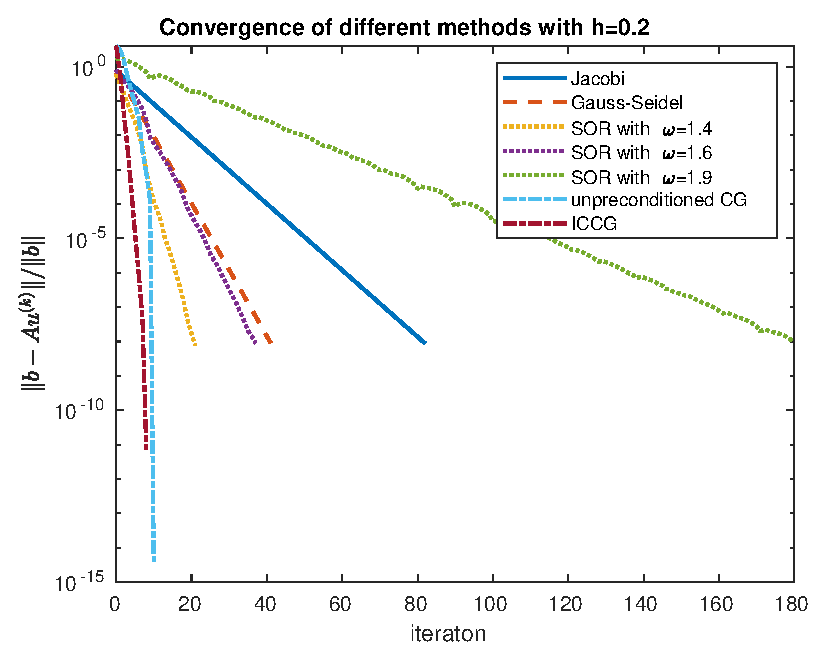
\includegraphics[scale=0.7]{h=0.2.eps}\\
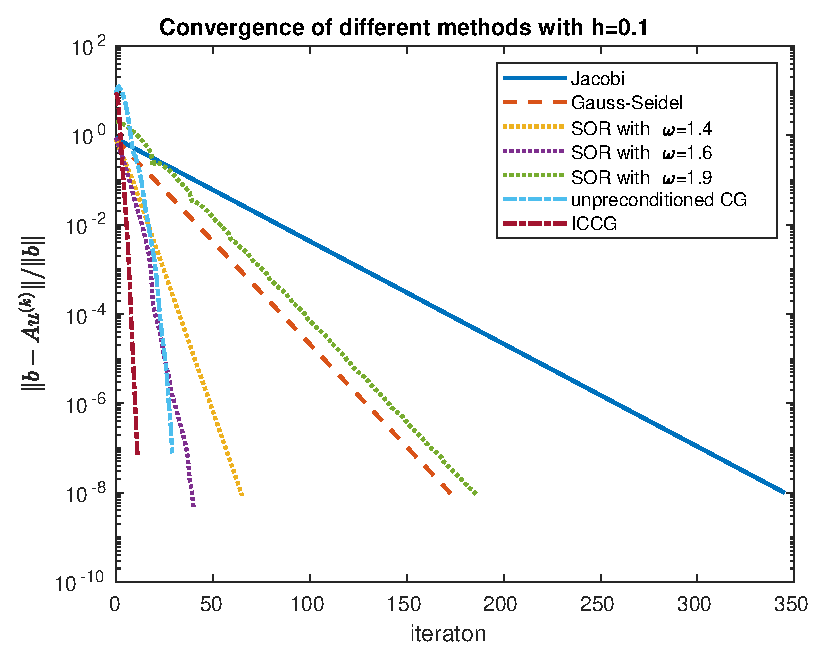
\includegraphics[scale=0.7]{h=0.1.eps}\\
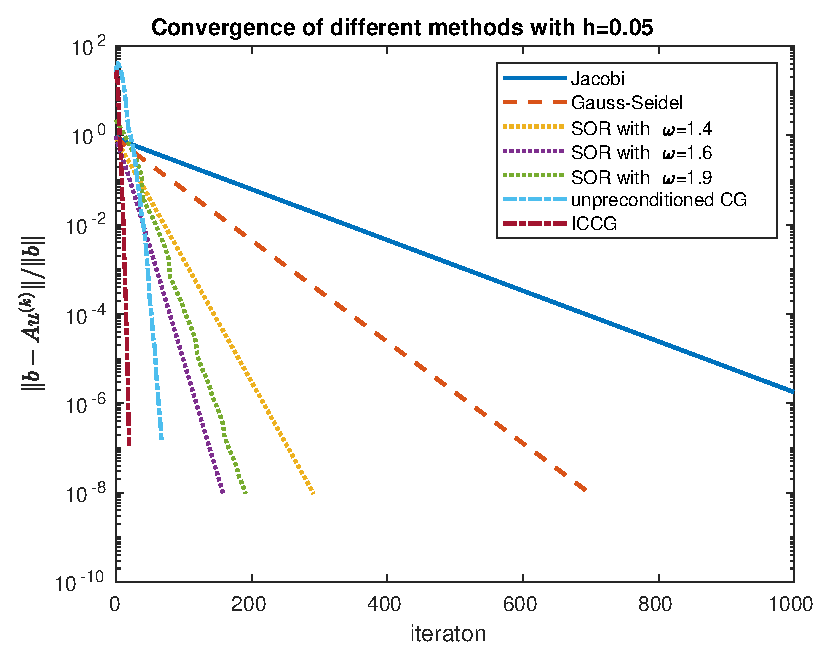
\includegraphics[scale=0.7]{h=0.05.eps}\\
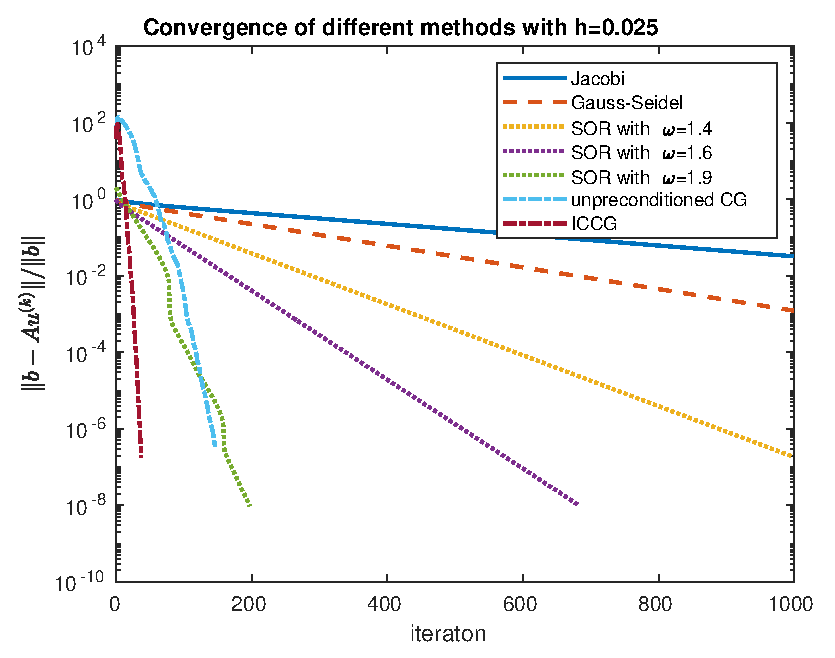
\includegraphics[scale=0.7]{h=0.025.eps}\\
\end{centering}
We observe that our optimal parameter $\omega$ for SOR seems to vary has $h$ changes, apparently approaching 2 as $h\to0$. The following table presents the number of iterations needed to converge under our tolerance for different methods and $h$ values.
\begin{table}[H]\centering
\begin{tabular}{|r|r|r|r|r|r|r|r|}\hline
{$h$}&{Jacobi}&{Gauss-Seidel}&{SOR ($\omega=1.4$)}&{SOR ($\omega=1.6$)}&{SOR ($\omega=1.9$)}&{CG}&{ICCG}\\\hline
0.2&83&42&22&38&181&10&8\\
0.1&346&174&66&41&187&29&11\\
0.05&1000&699&292&159&192&67&19\\
0.025&1000&1000&1000&684&198&146&37\\\hline
\end{tabular}
\end{table}
Noting that we cut $h$ in half each time, we now give the factor of increase in the number of iterations compared to the previous $h$ ($\text{iter}(h)/\text{iter}(2h)$).
\begin{table}[H]\centering
\begin{tabular}{|r|r|r|r|r|r|r|r|}\hline
{$h$}&{Jacobi}&{Gauss-Seidel}&{SOR ($\omega=1.4$)}&{SOR ($\omega=1.6$)}&{SOR ($\omega=1.9$)}&{CG}&{ICCG}\\\hline
0.1&4.1687&4.1429&3&1.0789&1.0331&2.9&1.375\\
0.05&{N/A}&4.0172&4.4242&3.8780&1.0267&2.3103&1.7273\\
0.025&{N/A}&{N/A}&{N/A}&4.3019&1.0312&2.1791&1.9474\\\hline
\end{tabular}
\end{table}
Both Jacobi and Gauss-Seidel grow like $\OO(h^{-2})$ while both CG and ICCG appear to be converging to growing like $\OO(h^{-1})$. The different SOR methods are trickier, but appear to be near constant for sufficiently large $h$ and converge to growing like $\OO(h^{-2})$ as $h$ becomes sufficiently small.

\section{Problem 3}
Consider a symmetric positive definite matrix $A$ that has one thousand eigenvalues
uniformly distributed between $1$ and $10$, and one eigenvalue of $10^4$ and another symmetric positive definite matrix $B$ that has an eigenvalue
of $1$ and has one thousand eigenvalues uniformly distributed between $10^3$ and $10^4$. First considering the case of matrix $A$, let the eigenvalues be ordered such that $\lambda_1\leq\ldots\leq\lambda_{n-1}\ll\lambda_n$ and consider the polynomial
\[
p_k(z)=\left(T_{k-1}\left(\frac{2z-\lambda_{n-1}-\lambda_1}{\lambda_{n-1}-\lambda_1}\right)\biggr/T_{k-1}\left(\frac{-\lambda_{n-1}-\lambda_1}{\lambda_{n-1}-\lambda_1}\right)\right)\frac{\lambda_n-z}{\lambda_n}.
\]
Note that the second term in this product is zero at $z=\lambda_n$, so 
\[
\max_{i=1,\ldots,n}|p_k(\lambda_i)|=\max_{i=1,\ldots,n-1}|p_k(\lambda_i)|.
\]
Then, letting $\kappa'=\lambda_{n-1}/\lambda_1\leq10$, we can apply (4.59) in the text to the first function in this product to get that
\[
\max_{i=1,\ldots,n-1}\left|T_{k-1}\left(\frac{2z-\lambda_{n-1}-\lambda_1}{\lambda_{n-1}-\lambda_1}\right)\biggr/T_{k-1}\left(\frac{-\lambda_{n-1}-\lambda_1}{\lambda_{n-1}-\lambda_1}\right)\right|\leq2\left(\frac{\sqrt{\kappa'}-1}{\sqrt{\kappa'}+1}\right)^{k-1}.
\]
Coupling this with the fact that the second term in our product is linear, we can apply (4.51) in the text to get that
\begin{align*}
\frac{\| e^{(k)} \|_{A}}{\| e^{(0)} \|_{A}}&\leq \max_{i=1,\ldots,n}|p_k(\lambda_i)|\leq2\left(\frac{\sqrt{\kappa'}-1}{\sqrt{\kappa'}+1}\right)^{k-1}\frac{\lambda_n-\lambda_1}{\lambda_n}\\&\leq
2\left(\frac{\sqrt{10}-1}{\sqrt{10}+1}\right)^{k-1}\frac{10^4-1}{10^4}=2*0.9999\left(\frac{\sqrt{10}-1}{\sqrt{10}+1}\right)^{k-1}.
\end{align*}
For matrix $B$, order the eigenvalues such that $\lambda_1\ll\lambda_2\leq\ldots\leq\lambda_n$ and consider the polynomial
\[
p_k(z)=\left(T_{k-1}\left(\frac{2z-\lambda_{n}-\lambda_2}{\lambda_{n}-\lambda_2}\right)\biggr/T_{k-1}\left(\frac{-\lambda_{n}-\lambda_2}{\lambda_{n}-\lambda_2}\right)\right)\frac{\lambda_1-z}{\lambda_1}.
\]
Note that the second term in this product is zero at $z=\lambda_1$, so 
\[
\max_{i=1,\ldots,n}|p_k(\lambda_i)|=\max_{i=2,\ldots,n}|p_k(\lambda_i)|.
\]
Then, letting $\kappa'=\lambda_{n}/\lambda_2\leq10$, we can apply (4.59) in the text to the first function in this product to get that
\[
\max_{i=2,\ldots,n}\left|T_{k-1}\left(\frac{2z-\lambda_{n}-\lambda_2}{\lambda_{n}-\lambda_2}\right)\biggr/T_{k-1}\left(\frac{-\lambda_{n}-\lambda_2}{\lambda_{n}-\lambda_2}\right)\right|\leq2\left(\frac{\sqrt{\kappa'}-1}{\sqrt{\kappa'}+1}\right)^{k-1}.
\]
Coupling this with the fact that the second term in our product is linear, we can apply (4.51) in the text to get that
\begin{align*}
\frac{\| e^{(k)} \|_{B}}{\| e^{(0)} \|_{B}}&\leq \max_{i=1,\ldots,n}|p_k(\lambda_i)|\leq2\left(\frac{\sqrt{\kappa'}-1}{\sqrt{\kappa'}+1}\right)^{k-1}\left|\frac{\lambda_1-\lambda_n}{\lambda_1}\right|\\&\leq
2\left(\frac{\sqrt{10}-1}{\sqrt{10}+1}\right)^{k-1}\frac{10^4-1}{1}=2*9999\left(\frac{\sqrt{10}-1}{\sqrt{10}+1}\right)^{k-1}.
\end{align*}
In attempting to analyze the convergence of CG for these matrices, it is important to note that we have not established the tightness of these bounds, so they may not give an accurate depcition of the convergence rates in the slightest. If we do assume that these bounds are sufficiently tight to give us information about the convergence rates, we expect CG to reduce relative error at the same rate of $\frac{\sqrt{10}-1}{\sqrt{10}+1}$ for both $A$ and $B$ in their respective norms; however, the bound on the convergence of $B$ is 10000 times that of $A$, so we expect CG to take longer to reach a set relative error when applied to $B$ instead of $A$.
\end{document}